\chapter{Rapport intérmédiaire : 27.10.2018 au 09.11.2018}

\section{Setup pour la prise de mesure}
Pour effectuer les mesures, il est nécessaire d'effectuer un certain nombre de mesure afin d'avoir un nombre acceptable de données. L'idée est de respecter le plan ci-dessous voir la figure \ref{fig:PlanMod}. Dans un premier temps, les mesures seront effectuée dans une seule moitié du laboratoire. 

Le point rond "M" représente le master, les points ronds "S" représentent les slaves et finalement les points carrés "E" représentent les espions. C'est sur ces derniers que les mesures seront effectuées. 

Il sera nécessaire de prendre 20 mesures sur chaque point. Comme uniquement la première moitié sera considéré les mesures seront faites sur 10 points différents donc 200 données seront à disposition. Une mesure consiste à changer de canal de 1 à 50 et de faire ensuite la moyenne. 

Ces données devront être construites des variables suivantes pour un espion: 
\begin{enumerate}
	\item La coordonnée réelle
	\item Mesures brute pour un canal
	\item Le signal RSSI pour un canal
	\item Erreur pour un canal
	\item le calcul de la coordonnée 
\end{enumerate}

\todo{Afficher ce que reçoit le soft python pour savoir ce qu'il y a exactement car pour le moment c'est un peu flou}

\begin{figure}[H]
	\begin{center}
		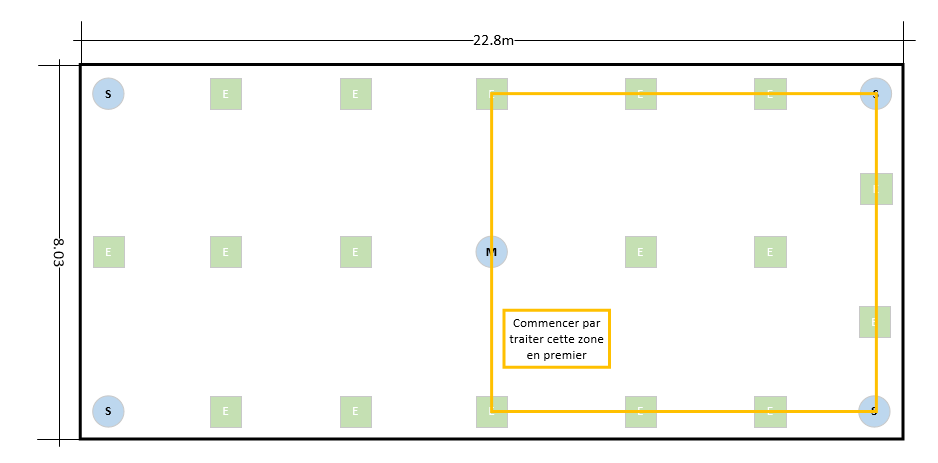
\includegraphics[scale=0.5]{figures/PlanMod.PNG}
		\caption{Montre le setup pour la prise de mesure}
		\label{fig:PlanMod} %% NOTE: always label *after* caption!
	\end{center}
\end{figure}

Le plan de la figure \ref{fig:PlanMod} et un simplification du plan réel de la figure \ref{fig:PlanRe}.

\begin{figure}[H]
	\begin{center}
		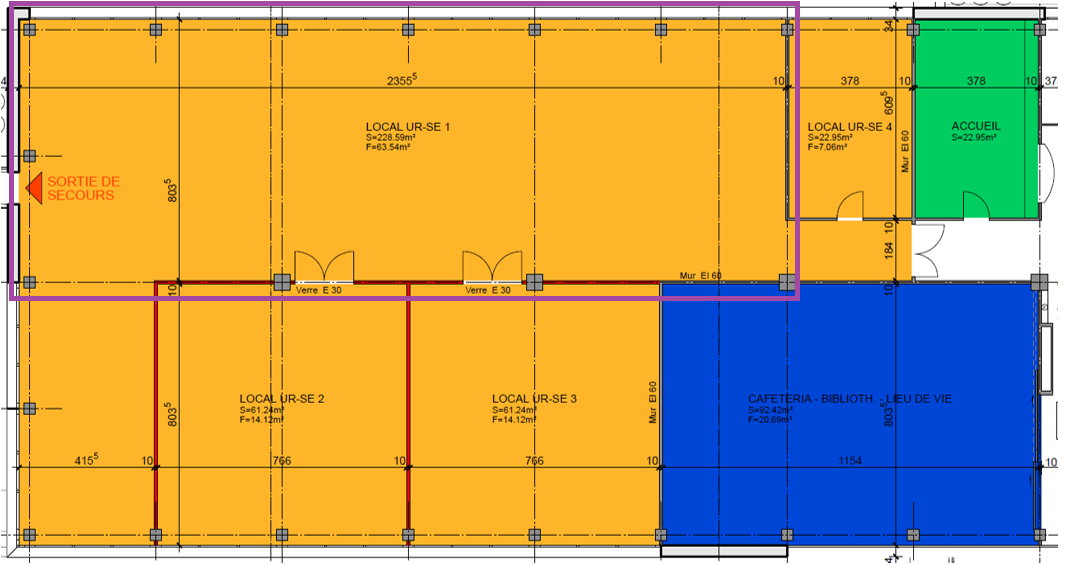
\includegraphics[scale=0.5]{figures/PlanRe.PNG}
		\caption{Montre le plan réel du laboratoire}
		\label{fig:PlanRe} %% NOTE: always label *after* caption!
	\end{center}
\end{figure}

\section{Reprise du soft python de Michael}
Le programme python est relié au Master du réseau LoRa. Il ordonne juste au master de faire un série de mesure. Dès que le master reçois une mesure, il passe le résultat au python qui le stock en RAM et fais passer ça dans des filtres Dans les données reçues, il y a le canal, la valeur brute de mesure, la RSSI, et l'erreur de fréquence estimée. Il est possible d'avoir les mesures brutes en lisant le logs, normalement elles se trouvent dedans (à vérifier).

Les RSSI sont pour l'échange maitre-escalve mais le spy mesure également un RSSI (probablement un rssi moyen).

Le master récupère toutes les mesures du spy et les transmet au PC. Il y a une partie mesure et une partie transmission. C'est ca qui fait que le protocol est un peu compliqué. Le spy stock dans sa RAM les mesures et ressort tout quand le master le demande. Ca c'est le python qui ordonance tout et c'est le fichier de config qui définit comment.

Les coordonnées sont calculées au niveau du soft python et en fonction de ce qui est rentré comme mesure, cela va dans le PositionSolver.

Il est normalement pas nécessaire de s'occuper du soft embarqué par contre il faut maîtriser les adresses.

Comme nous n'avons pas la dernière version du chip il est possible qu'il y ait certain bugs...

Selon le fichier de config, les mesures sont faites sur plusieurs canaux randomisés (ranging slot number = 40). Ca veut dire en gros 40 canaux et le soft python fait cela : 

\begin{enumerate}
	\item Mesurer sur 40 canaux sur un escalve
	\item Récuperer les data sur les spy
	\item mesurer le deuxième exclave
	\item Récupérer les valeurs
	\item etc...
\end{enumerate}

Si plusieurs spy : \\
mesure esclave 1 ->récupérer  spy1,spy2, sp3 / mesure esclave 2 ->récupérer  spy1,spy2, sp3. Les spy sont indépendant des mesures, ils font que écouter les mesures

La structure et datas reçue dans le python sont là :

\begin{lstlisting}
def new burst available(burst_list) :
'''
Callback when new bursts are available
:param burst_list: list_of_bursts
:return: None

=> It will calculate nodes new positions
'''
for burst in burst list:
position solver.update position_solver(burst)
system_gui.update_burst_info(burst)
\end{lstlisting}

C'est le callback qui est reçu dans lr24\_resolver.py. C'est une liste de burst (en python). C'est une liste d'obket "Burst". Et en gros ca stock toutes les mesures pour un couple master-escalve

Dans ces burst il y a les mesures brutes/ le rssi et l'erreur et ca filtre les piques(le bug du chip)
 
\begin{lstlisting}
for burst in burst list:
	valeurs = burst.values
\end{lstlisting}

valeurs[0, canal] = mesure brute pour un canal donné\\
valeurs[1, canal] = rssi pour un canal donné\\
valeurs[2, canal] = erreur pour un canal\\

Pour effectuer les mesures il y a un bouton start/stop.

Il y a deux dimension pour juste un couple maitre escalve. Après c'est N x éenombre. Deux dimensions car canaux x [ raw, rssi, erreur]

%\begin{lstlisting}
% for i=0 to Array.length(t)-1 do
%\end{lstlisting}


%\begin{enumerate}
%	\item fgfd
%	\item gdgfd
%\end{enumerate}


%\begin{figure}[H]
%	\begin{center}
%		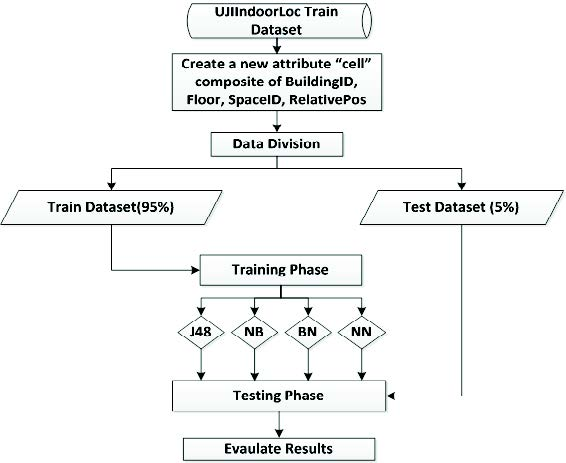
\includegraphics[scale=1]{figures/newattribute.jpg}
%		\caption{The new attribute “cell” construction phase}
%		\label{fig:newAttribute} %% NOTE: always label *after* caption!
%	\end{center}
%\end{figure}

%\todo{Compléter cette partie qui semble importante}

